%%%%%%%%%%%%%%%%%%%%%%%%%%%%%%%%%%%%%%%%%%%%%%%
%
% Template per Elaborato di Laurea
% DISI - Dipartimento di Ingegneria e Scienza dell’Informazione
%
% update 2015-09-10
%
% Per la generazione corretta del 
% pdflatex nome_file.tex
% bibtex nome_file.aux
% pdflatex nome_file.tex
% pdflatex nome_file.tex
%
% article
% Required fields: author, title, journal, year. 
% Optional fields: volume, number, pages, month, note.
%@article{donoho,
%  author = {Donoho D. L.},
%  title = {Compressed Sensing},
%  journal = {IEEE Trans. Inf. Theory},
%  volume = {52},
%  number = {4},
%  pages = {1289-1306},
%  year = {2006}
%}

% conference
% same as inproceedings
% Required fields: author, title, booktitle, year. 
% Optional fields: editor, volume or number, series, pages, address, month, organization, publisher, note
%@conference{dalal,
%  author = {Dalal N., Triggs B.},
%  title = {Histograms of Oriented Gradients for Human Detection},
%  booktitle = {Computer Vision and Pattern Recognition (CVPR)},
%  address = {San Diego, USA},
%  year = {2005},
%  month = {20-26 June},
%  pages = {886-893}
%}

% website
% as misc
% Required fields: none. 
% Optional fields: author, title, howpublished, month, year, note.
%@misc{ictbusiness,
%  title = {ICT business},
%  howpublished = {http://www.ictbusiness.it/},
%  note = {ultimo accesso 15/06/2015}
%}
%%%%%%%%%%%%%%%%%%%%%%%%%%%%%%%%%%%%%%%%%%%%%%%

% formato FRONTE RETRO
\documentclass[epsfig,a4paper,10pt,titlepage,twoside,openany]{report}
\usepackage{epsfig}
\usepackage{plain}
\usepackage{setspace}
\usepackage[paperheight=29.7cm,paperwidth=21cm,outer=1.5cm,inner=2.5cm,top=2cm,bottom=2cm]{geometry} % per definizione layout
\usepackage{titlesec} % per formato custom dei titoli dei capitoli
\usepackage{xcolor}
\usepackage{subfig}
\usepackage{wrapfig}
\usepackage{gensymb} %to use \degree symbol
\usepackage{amsmath}
\usepackage{amsfonts}
\usepackage{multirow}

%%%%%%%%%%%%%%
% \usepackage[latin1]{inputenc} % per Windows;
\usepackage[utf8x]{inputenc} % per Linux (richiede il pacchetto unicode);


% two lines to have subsubsections in the table of contents
\setcounter{secnumdepth}{3}
\addtocontents{toc}{\setcounter{tocdepth}{3}}

\singlespacing

\usepackage[english]{babel}

\begin{document}

  % nessuna numerazione
  \pagenumbering{gobble} 
  \pagestyle{plain}

\thispagestyle{empty}

\begin{center}
  \begin{figure}[h!]
    \centerline{
\psfig{file=marchio_unitrento_colore_it_202002.eps,width=0.6\textwidth}}
  \end{figure}

  \vspace{2 cm} 

  \LARGE{Department of Engineering\\}

  \vspace{1 cm} 
  \Large{Artificial Intelligence Systems}

  \vspace{2 cm} 
  \Large\textsc{Final Report\\} 
  \vspace{1 cm} 
  \Huge\textsc{Image Recapturing\\}
%  \Large{\it{Sottotitolo (alcune volte lungo - opzionale)}}


  \vspace{2 cm} 
  \begin{tabular*}{\textwidth}{ c @{\extracolsep{\fill}} c }
      \Large{Supervisors} & \Large{Students}\\
      \Large{DE NATALE Francesco} & \Large{GUGLIELMI Matteo} \\
      \Large{VERDE Sebastiano} & \Large{MAZZARO Roberto} \\
      & \Large{RECH Antonella}
  \end{tabular*}

  \vspace{2 cm} 
  
  \begin{center}
    \Large{Academic Year : 2021/2022}
  \end{center}
  
\end{center}


  \clearpage
  
  % inizio numerazione pagine in numeri arabi
  \mainmatter

    % indice
    \tableofcontents
    \clearpage
    
    
          
    % gruppo per definizone di successione capitoli senza interruzione di pagina
    \begingroup
      % nessuna interruzione di pagina tra capitoli
      % ridefinizione dei comandi di clear page
      \renewcommand{\cleardoublepage}{} 
      \renewcommand{\clearpage}{} 
      
      \titleformat{\chapter}
        {\normalfont\Huge\bfseries}{\thechapter}{1em}{}
        
      \titlespacing*{\chapter}{0pt}{0.59in}{0.02in}
      \titlespacing*{\section}{0pt}{0.20in}{0.02in}
      \titlespacing*{\subsection}{0pt}{0.10in}{0.02in}
      
      % sommario
      % \input{sommario}
   
      % lista dei capitoli
      \newpage
      \paragraph{Abstract}
Nowadays, with the availability of sofisticated digital cameras, images can be acquire with high-quality also from LCD monitor screens quite easily. In light of this, an hypothetical attacker may want to reacpture a forged image in order to hide imperfections and to increase its authenticity.\\
The underlying idea of this work is to develop an algorithm, following a piece of the paper cited in the bibliography \cite{paper}, which is able to recognize whether a specific image has been recaptured or not. \\
As quoted in the reference article, the authors address that '[...] aliasing and blurriness are the least scene dependent features'; since aliasing can be ereased by setting the parameters of the recapturing system to predetermined values, in this work we focus on the bluriness feature in order to perform the final recognition. More precisely, a set of learned edge bluriness are used to perform a classification of each input image.\\
Every time a scene is captured with a digital camera, a certain amount of blur is introduced into the picture by the image acquisition system. This blur can be characterized by the so called Point Spread Function of the capture device. Unfortunately, the PSF of a system is not easily achievable and the Line Spread Function (LSF) is used instead. 'By definition, a line spread function is a $1-$D function
corresponding to the first derivative of the edge spread function (ESF)' \cite{bluriness}\\
Another important component are the two over-complete dictionaries built by means of the K-SVD algorithm, one for both recaptured and single captured images in the available dataset \cite{database}. Each dictionary is trained to provide an optimal sparse representation of the Line Spread Profile function extracted from the example images. The purpose of the two dictionaries is to describe how well wach dictionary fits the line spread profile matrix ($Q_i$) of a query image. In poor words, an approximation error is computed as a measure of likeliness between an unknown query image and $D_{SC}$ and $D_{RC}$.\\
These dictionary, which will be referred to as $D_{SC}$ and $D_{RC}$ for the dictionary trained with single captured and recaptured images respectively, have a key role the approximation error which is one of the two features used.\\ The other feature used, $\lambda_{avg}$, refers to the average of Line Spread Profile widths computed as follows : the value of $\lambda$ is defined as the minimum distance of the ESF such that at least $95\%$ of the spectral energy of the spread function falls within it. \\
Eventually, after having computed $\lambda_{avg}$ and $E_d$ for every image of the training set, a support vector machine classifier (SVC) is trained.\\
Whenever an unknown query image has to be classified, the aforesaid features has to be computed and then feed the already built SVM with the respective values.
      \newpage
      \chapter{Implementation}
The developped algorithm is written in Python coding language.\\
It was deemed appropriate to subdivide the whole script in five main modules in order to have a clean and modular package. This also allows for saving files with intermediate results to save computational power since some processes are very demanding.\\
Enumerating the modules :
\begin{itemize}
    \item \textbf{dataset split} into training and test set;
    \item \textbf{calculus} of the Line Spread Profile matrix \textbf{$Q_i$} for every image;
    \item \textbf{building} of the over-complete \textbf{dictionaries} $D_{SC}$ and $D_{RC}$;
    \item SVM \textbf{training}
    \item address the performane of the \textbf{SVC testing} it on the test set.
\end{itemize}
\paragraph{How to use} Sequence of action in order to make this code work:
\begin{enumerate}
    \item run 'phase1$\_$QiCalculusdataset.py' (no need to do that because they are already computed in the given complete$\_$dataset folder) : compute all the matrices for each camera and type of image;
    \item run 'dataset$\_$acquisition$\_$txt.py' : perform the training and test sets formation;
    \item run 'make$\_$dictionary$\_$from$\_$txt.py' or 'make$\_$dictionary$\_$from$\_$txt$\_$.py' : the only difference here is that in the first module the building process start with complitely empty dictionaries; instead in the second one, dictionaries are initialized;
    \item run 'SVM$\_$training.py' : compute and save the hyperplane equation which better  separates the plane linearly;
    \item run 'SVM$\_$classifier.py' : saves significant statistics about achieved performances ;
\end{enumerate}
\section{Dataset formation}
This module automatically splits the whole dataset into training and test set as explained in the \textit{Section VI-A} of the reference paper \cite{paper}.\\
As specified in the latter :
\begin{itemize}
    \item for single captured images, $15$ randomly chosen images are selected for training purposes;
    \item concerning recaptured images, for every pair of cameras involved, where the first one is the device used to capture the original image and the second one the system used to recapture it, we randomly select $3$ pictures for training purposes.
\end{itemize}
The remaining ones, both for recaptured and single captured images, are kept for performance testing.\\
For each camera, both in single captured and recaptured images, the outputs are two .txt files containing the paths of the Line Spread Profile matrices for training and test images respectively.
\section{$Q_i$ Calculus}
    In this section we implement the method described in the paper \cite{paper} for the calculus of the matrix $Q$.\\
    The proposed process determines, for any given single or recaptured image, a LSP matrix $Q_i$. 
    Since this part is very computationally demanding, we stored the resulting matrices in the corresponding directory of each camera model to used them later on in the next steps.\\

    The feature matrix extracted for each dataset's image contains the LSP of any columns presents in the selected blocks. We achieved these blocks by applying the following criterion, explained in details in the paper :
    \begin{itemize}
        \item firstly, the query image is converted to greyscale and all edges contained in the image are detected using a Canny Edge Detector (Canny Filter);
        \item the query image is, then, divided into non-overlapping blocks $B(m,n)$ of size $W \times W$ with $W=16$ pixels;
        \item then, we check for horizontal, near horizontal, vertical and near vertical single edges and the blocks are chosen by counting the number of columns containing only one non-zero value. A block is considered only when the condition $\eta \geq \beta W$ is satisfied, where $\beta=0.6$;
        \item the LS function $q_i$ is then calculated by normalizing the gradient of each columns given the previously obtained blocks. Subsequently, all the $q_i$s are interpolated by $4 \times$ to increase the number of data points to $64$;
        \item to determine the $\lambda_{avg}$, we compute the distance that embeds the $90\%$ of the spectral energy of each interpolated column of the $Q_i$ matrix. Consequently, we compute the mean of those distances;
        \item at this level, only the greylevel blocks, which meet some contraints, are selected and the corresponding interpolated $q_i$ inserted in the $Q_i$ matrix of the image. These contraints are :
        \begin{itemize}
            \item the block-based variance $\sigma_{m,n}$ has to fall within the largest $20\%$ of all the computed values;
            \item the average lambda's value $\overline{\lambda}_{m,n}$ has to fall between the smallest $10\%$ of all the computed values.
        \end{itemize}
    \end{itemize}
    From now on, the Line Spread matrices for recaptured and single captured images are stored and they wll be used for training purposes.
\section{Dictionary building}
This script perform dictionary learning \cite{omp}. Given the training feature matrix S, which is obtained by the horizontal composition of all the previously computed $Q_i$, the goal of this technique is to obtain the best sparse dictionary, D $\in \mathbb{R}^{W \times K}$, that provides an optimal sparse representation for all the LSP matrices in S.\\
Once the matrix S has been built, a very large matrix is obtained. In order to reduce its size, a sort of resizing operation is applied : the training feature matrix is obtained by keeping only one column out of four in the original matrix.\\
The result is used to fed the \textit{K-SVD algorithm} whose main parameters are briefly discussed in the following sections (\ref{cha:ksvd}) \\
Since the whole process requires a consistent amount of time, once both $D_{SC}$ and $D_{RC}$ have been built, they're saved in a .txt file. Doing so, they just have to be loaded in the program when they're needed later on.

\subsection{K-SVD Parameters}
\label{cha:ksvd}
In our implementation, we used the K-SVD function provided by the sklearn library even though we hard coded an alternative version which turned out to be a little less efficient.\\
This function takes as inputs some specific parameters which define the characteristics the output has to meet. Unfortunately, the \textbf{reference paper doesn't clearly specify the parameters}, same for the SVM implementation, so we had to make several trials in order to find a set of values which lead to a decent overall result. \\
More precisely, the parameters to be specified are :
\begin{itemize}
    \item \textit{Number of components} : number of elements the output dictionary contains. Those ones may be zero or non-zero valued elements depending on the grade of sparsity defined (see below). The exact number is not defined in the paper so we sought a value which may represent a good trade-off between quality and computational demand.\\In the final implementation we set this parameter to $50$ but increasing the number of components may likely lead to better results;
    \item \textit{Alpha} : consists in the sparsity controlling parameter. Reading the paper, at first it seems it has to be set to $0$ but, with this particular value, the obtained results are very low in quality. Guessing an alpha parameter equal to $1$ we observed a consistent increse in quality performance;
    \item \textit{Maximum number of iterations} : integer number which indicates an upper bound on the number of iteration to perform. In the reference paper \cite{paper} it is clearly specified to use $160$;
    \item \textit{Tollerance} : tollerance for numerical error. As defualt is to $10^{-8}$. In this case we used $10^{-6}$ as shown in a similar purpose algorithm developed in MathLab;
    \item \textit{Transformation algorithm} : algorithm to process the data. We used the OMP algorithm, as specified in the reference paper, to estimate the sparse solution:
    \item \textit{Number of non-zero coefficients in the transformation} : number of non-zero coefficients to the target for each column of the solution. This corresponds to the degree of sparsity of the output, in this specific case of the two dictionaries. This parameter in the reference paper is named as $L$ an indicates the optimal number of atoms in the dictionaries. It is explained that this parameters is set to $3$ because it coincide with the peak of the second derivative for our training sets.
\end{itemize}

\subsection{Dictionary initialization}
As explained in section $VI-A$ of the reference paper 'The initial set of atoms was constructed from the Line Spread functions of the nine single capture cameras and 63 different LS functions determined from randomly selected image recapture camera combinations'. We actually implement this part but we have not noticed any significant difference.
\section{Support Vector Machine}
\subsection{Training phase}
After having extracted the aforesaid features, as indicated in the followed paper \cite{paper}, a support vector machine (SVM) has been used in order to classify unknown images.\\
The kernel used is of the linear kind and the training phase has been structured as follows :
\begin{itemize}
    % \item the path of every image, recaptured and single captured ones, has been extracted and stored in different lists one for each camera model;
    % \item at this point a random split has been performed as specified in the aforesaid paper:
        % \begin{itemize}
            % \item concerning the single captured images, $15$ images are kept for training purposes;
            % \item for the recaptured examples, the training set's size is set to $3$.
        % \end{itemize}
        % At the end of this point, all the training and test lists of each camera are put together obtaining two lists respectively conatining training and test samples' paths. \\
        % More specifically, four lists have to be obtained : 
        % \begin{enumerate}
            % \item training list for recaptured images with with $3$ elements;
            % \item training list for single captured list woth $15$`';
            % \item test list for recaptured images;
            % \item test list for single captured images.
        % \end{enumerate}
    \item paths of images used for training purposes are stored in two separated lists, both for recaptured and single captured;
    \item pre-computed dictionaries are loaded;
    \item iteratively, for each element within the two lists : 
        \begin{itemize}
            \item the corresponding already calculated list of $Q_i$ is loaded;
            \item the features (approximation error $E_d$ and average line spread function width $\lambda_{avg}$) are computed and saved within a common Pandas DataFrame [\textbf{Picture} \ref{fig:table_csv}] organized in columns as follows:
          \begin{itemize}
              \item first column : it's composed by integer indexes;
              \item second column : it's formed, cell by cell, by the path of a specific processed image;
              \item third column : it contains the true label of a specific image;
              \item fourth column :  it displays the computed values of $\lambda_{avg}$ for the corresponding image;
              \item fifth and last column : element-wise, it showcases approximation errors.
          \end{itemize}
        \end{itemize}
          It's worth mentioning that the previously calculated $Q_i$ and dictionaries are loaded in order to save some computational power;
    \item at the end, a unified csv table made of training samples including both recaptured and single captured values, is used to train the SVM. Once the fitting has finished, the resulting model is saved in preparation for future predicting operations.
\end{itemize}

\begin{figure}[h!]
    \centering 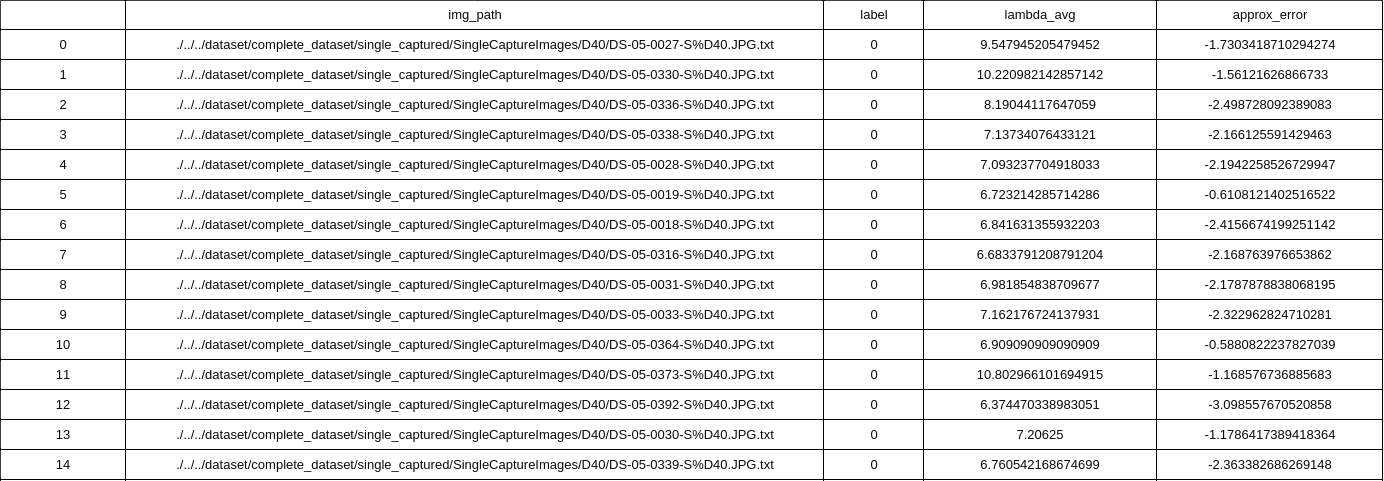
\includegraphics[width=\textwidth]{Images/table.png}
    \caption{Pieces of Panda DataFrame table in .csv file format.}
    \label{fig:table_csv}
\end{figure}

\subsection{Classification}
At this level of implementation, the SVM has already been trained and the model stored.\\
This part of implementation consists of testing the SVM on the test set in order to adress its performances.\\
By analogy with the training phase, this part's explanation is structured in points as well :
\begin{itemize}
    \item the first step consists in extracting the path of all images used for test, both recaptured and single captured, shot by all the cameras;
    \item for each picture, the feature extraction process is performed and the ouput is saved within a .csv file equivalently to the training part;
    \item consequently, a predition is carried out on each image and the results are showed in a table which exhibits: the amount of correctly and erroneously classified rate and the accuracy achieved for each camera model.\\
          Furthermore, the confusion matrix for each camera is video-printed, where :
          \begin{itemize}
              \item the first element represents the True Negatives (images correctly classified as Single Captured);
              \item the first element represents the False Negatives (images wrongly classified as Single Captured);
              \item the first element represents the True Positives (images correctly classified as Recaptured);
              \item the first element represents the False Positives (images wrongly classified as Recaptured);
          \end{itemize}
            It is noteworthy to adress that in order to obtain independent statistics, the classification process is performed separately on each camera model's test set.
\end{itemize}

      \newpage
      \chapter{Conclusions}
\paragraph{General results overview}
The obtained results are not as good as the ones presented in the paper \cite{result} but it was expected since usually the shown results are obtained with the omission of some particulars, sometimes important, e.g. missing parameters.\\
Concerning the recaptured images, the final results on the test set are worse than the expected values. However, the divergence between presented and achieved accuracies is not that large. Indeed, for certain camera models we achieve a classification accuracy of $95\%$ and $97\%$ in the best cases and of $80\%$ and $78\%$ in the worst cases.\\
As average recognition accuracy, for the recaptured images we obtained an $88\%$ of correct classification rate against an expected $99.03\%$.\\
Results of lower quality are obtained when trying to recognize single captured images; in this case the best accuracy achievable is around $80\%$ with an average of $56\%$ against the expected $94.89\%$.\\

\paragraph{Analysis on the camera models}
Along the paper has been explained that cameras provided with cheaper or older sensors perform poorely because their pictures are less sharp than most recent digital ones. In light of this, as expected, for low-cost cameras such as Kodak V550B, V550S and V610
we obtained lower accuracies, still considerably lower than the presented ones in the reference paper.\\
Eventually, we were surprised to see that TZ7 model performed badly in our algorithm while it's within the bests on according to the results shown in the paper.

\paragraph{Reasons for the differencies}
Some possible reasons for the observed differences in the final results, compared to the ones presented in the paper, may be the following ones :
\begin{itemize}
    \item ambiguity of the paper :
    \begin{itemize}
        \item sometimes, some steps are not clear enough in order to deeply understand the specific operation the authors make. In other words, they leave the door open to free interpratation of what they write leading to ambiguity and confusion when implementing a code;
        \item the lack of parameters indication, i.e. for the dictionary learning algorithm most of the parameters are missing and we had to assume some random values. It would have been possible to execute a grid search but, since the whole program implies a large amount of time, this wasn't possible. \\
              Another unclear point is how they initialize the sparse dictionaries because, in our case, we did not observed significant improvements doing so.
    \end{itemize}
\end{itemize}
      
    \endgroup


    % bibliografia in formato bibtex
    %
    % aggiunta del capitolo nell'indice
    \addcontentsline{toc}{chapter}{Bibliografia}
    % % stile con ordinamento alfabetico in funzione degli autori
    \bibliographystyle{acm}
    \bibliography{biblio}

\end{document}
